\chapter{组件-事件知识图谱表示学习}\label{chapter-3}
在已有的知识库中(如FB15K\cite{bordes2013translatingE}和YAGO37\cite{guo2018knowledge}),由于每个三元组$\left(head, relation, tail\right)$都可以视作一条知识而单独存在,知识图谱可以用多个三元组组成的集合表示,即 $\mathcal{KG}=\left\{\left(e_{i}, r_{k}, e_{j}\right)\right\}$(其中$i$、$j$为实体索引,$k$为关系索引)。因此,已有的大多数知识表示模型都是输入三元组$\left(head, relation, tail\right)$,然后着重于缩短这三者嵌入表示之间的语义距离。

在本文的组件-事件知识图谱$G=(\mathcal{F}, \mathcal{V}, \mathcal{E}, \mathcal{R})$中,每个组件-事件知识图谱都对应着一个故障类型$\mathcal{F}$,这使得每个三元组的成立与其上下文背景信息有关,且每个实体在不同的上下文中应有不同的嵌入表示,即应随着上下文的变化而动态地表示。详细分析如章节\ref{backgroud-analysis}所示。

虽然文献\parencite{feng2016gake,shi2017knowledge}尝试将图结构上下文引入嵌入表示,但是它们都将原本的图结构转为邻居上下文、路径上下文再进行嵌入表示学习。这种方式不足以获取全面的图结构上下文信息,且不能满足动态的嵌入表示学习,即不能根据具体上下文给同一实体不同的嵌入表示。
% 所以本文利用图神经网络获取组件-事件知识图谱中的上下文结构信息,再结合实体的语义信息,获取动态的实体嵌入表示。

为了满足实体随上下文动态表示,本章主要设计了针对组件-事件知识图谱的知识表示学习模型,并分为3节展开介绍。首先,本章进行了场景分析,罗列了组件-事件知识图谱进行表示学习时要解决的问题。然后详细介绍了针对组件-事件
知识图谱的表示学习模型。最后,本章设计了详细的实验验证本文模型的有效性。
\section{场景分析}\label{backgroud-analysis}
% GCN  RGCN  SACN KBAT
本节主要分析了组件-事件知识图谱的特性,解释了为何本文的知识表示学习与上下文背景信息相关,且需要动态的嵌入表示。

\subsection{上下文背景信息}\label{context-analysis}
在组件-事件知识图谱中,一个三元组的成立与其上下文拓扑关系有关,这使得一个三元组不能被视为一条可以单独存在的知识。下面是以图\ref{graph-example}中信息为例,对组件-事件知识图谱中三大类关系的分析:

(1)抽象事件间的因果关系。以三元组$\left(Backoff, cause, HttpServerError Exception 503\right)$为例,该三元组中$Backoff$(微服务重启失败)和$HttpServerError 503$(微服务服务不可用)之间不一定有触发关系。该三元组的成立,需要一定的背景信息如式\ref{event-event-relation}所示。
% ,即需要这两个事件发生在同一个微服务组件、或者有交互依赖关系的两个微服务组件。
\begin{equation}
    \begin{aligned}
        &\left ( ts-train-service, happen, Backoff \right ) \\
        &\wedge \left ( ts-ticketinfo-service, happen, HttpServerError Exception 503 \right ) \\
        &\wedge \left ( ts-ticketinfo-service, call, ts-train-service \right ) \\
        &\Rightarrow \left ( Backoff, \boldsymbol{cause}, HttpServerError Exception 503 \right )
    \end{aligned}
\label{event-event-relation}
\end{equation}

% 1)事件到事件的因果关系。以预测三元组中尾实体$\left(Backoff, cause, \textcolor[rgb]{1,0,0}{?}\right)$为例,推理关系如式\ref{event-event-relation-entity}所示,即需要这两个事件发生在同一个微服务组件、或者有交互关系的两个微服务组件。
% \begin{equation}
%     \begin{aligned}
%         &\left ( ts-train-service, happen, Backoff \right ) \\
%         &\wedge \left ( ts-ticketinfo-service, happen, HttpServerError Exception 503 \right ) \\
%         &\wedge \left ( ts-ticketinfo-service, call, ts-train-service \right ) \\
%         &\Rightarrow \left ( Backoff, \boldsymbol{cause}, HttpServerError Exception 503 \right )
%     \end{aligned}
% \label{event-event-relation-entity}
% \end{equation}

(2)组件到抽象事件的发生关系。以三元组$(ts-travel-service, happen, HttpServerError Exception 500)$为例,该三元组中$ts-travel-service$是否会发生事件$HttpServerError$$Exception 500$同样与其周边设备的状态有关。该三元组成立依据于式\ref{event-device-relation}中所示的条件。
\begin{equation}
    \begin{aligned}
        &\left ( ts-ticketinfo-service, happen,  HttpServerError Exception 503\right ) \\
        &\wedge \left ( ts-travel-service, call, ts-ticketinfo-service \right ) \\
        &\wedge \left ( HttpServerError Exception 503, cause, HttpServerError Exception 500 \right ) \\
        &\Rightarrow \left ( ts-travel-service, \boldsymbol{happen}, HttpServerError Exception 500 \right )
    \end{aligned}
\label{event-device-relation}
\end{equation}

(3)组件到组件的交互关系。以三元组$\left( container1, hold, ts-train-service \right)$为例,该三元组中$container1$负载着$ts-train-service$而不是其他微服务,同样需要借助背景信息才能推导出来。背景信息推导出该三元组成立的过程,如式\ref{device-device-relation}所示。
\begin{equation}
    \begin{aligned}
        &\left ( container1, happen,  cpu 100\% \right ) \\
        &\wedge \left ( container1, happen,  memory 100\% \right) \\
        &\wedge \left ( ts-train-service, happen,  Backoff \right) \\
        &\wedge \left ( cpu 100\%, cause,  Backoff \right) \\
        &\wedge \left ( memory 100\%, cause,  Backoff \right) \\
        &\Rightarrow \left ( container1, \boldsymbol{hold}, ts-train-service \right )
    \end{aligned}
\label{device-device-relation}
\end{equation}

由上述分析可见,组件-事件知识图谱中每条三元组都不能作为一条知识单独存在,而是知识图谱中三元组之间相互佐证使得整个拓扑图成为了蕴含知识的知识图谱。由此启发,组件-事件知识图谱的知识表示学习需要将实体所在上下文背景信息考虑进去,才能学习得到有效的实体与关系嵌入表示。
% 在组件-事件知识图谱表示学习中,需要考虑三元组的上下文。
% 已有的方式
% 引入逻辑规则,在传统的知识图谱中,关系都有丰富的语义信息(与常识知识有关),可以根据语义信息生成一些推理规则。比如
% isMarriedTo(x,y)->isMarriedTo(y,x)
% hasChild(x,y)且isCitizenOf(y,z)->isCitizenOd(x,z)
% playsFor(x,y)->isAffiliatedTo(x,y)
% 在组件-事件知识图谱中,只有因果关系,产生关系和交互关系,语义信息不足,生成的规则不具有通用性。规则是否成立其与具体的拓扑关系、抽象事件类型、组件类型都有关系。比如\ref{graph-example}中从“微服务ts-train-service发生BackOff就会导致请求它的微服务ts-ticketinfo-service发生HttpServerError”可以生成规则“微服务x发生BackOff就会导致请求它的微服务y发生HttpServerError”。该条规则只在当前的分布式应用可用,随着应用更新(添加了备用的微服务ts-train-service2或者开发人员添加异常处理使之不报错)或在其他的两个有访问关系的微服务之间,该条规则就会不适用。一方面规则需要大量人工编写审核,一方面即使自动生成规则也没有通用性,所以引入规则进行知识表示学习不可行。
\subsection{动态嵌入表示}
根据\ref{context-analysis}节分析,本文知识图谱表示学习需要引入上下文背景信息。在引入上下文背景信息方面,文献\parencite{feng2016gake,shi2017knowledge}将实体所在的图结构转为邻居上下文、路径上下文,通过最大化实体在其上下文的条件概率进行嵌入表示学习。但这种最大化概率的方式,对实体、关系的嵌入表示是静态的,即一旦训练完成嵌入表示是不会再随着上下文改变的。

这种获取静态嵌入表示的方法不适用于组件-事件知识图谱的表示学习。因为同一抽象事件由于其所在上下文不同、所在设备不同应当有着不同的嵌入表示。如图\ref{order-service-error}所示是"订票服务不可用"故障对应的组件-事件知识图谱部分示意图,在该图中同样存在$Backoff$抽象事件和$\left(ts-travel-service, happen, HttpServiceError Exception 500\right)$三元组,但该图中$ts-travel-service$发生$HttpServiceError Exception 500$是由于订票微服务$ts-order-service$上发生的抽象事件$Backoff$导致的。相对应的图\ref{graph-example}中$ts-travel-service$发生$HttpServiceError Exception 500$是微服务$ts-train-service$上的$Backoff$间接导致的,对应着"数据库不可用无法查票"故障。在这两个故障场景中,抽象事件$HttpServiceError Exception 500$是由不同原因导致的,所以应有不同的嵌入表示。抽象事件$Backoff$发生在不同的微服务上,也应有着不同的嵌入表示。所以,在组件-事件知识图谱中,实体嵌入表示需要随上下文信息动态变化。
\begin{figure}[htbp]
    \centering
    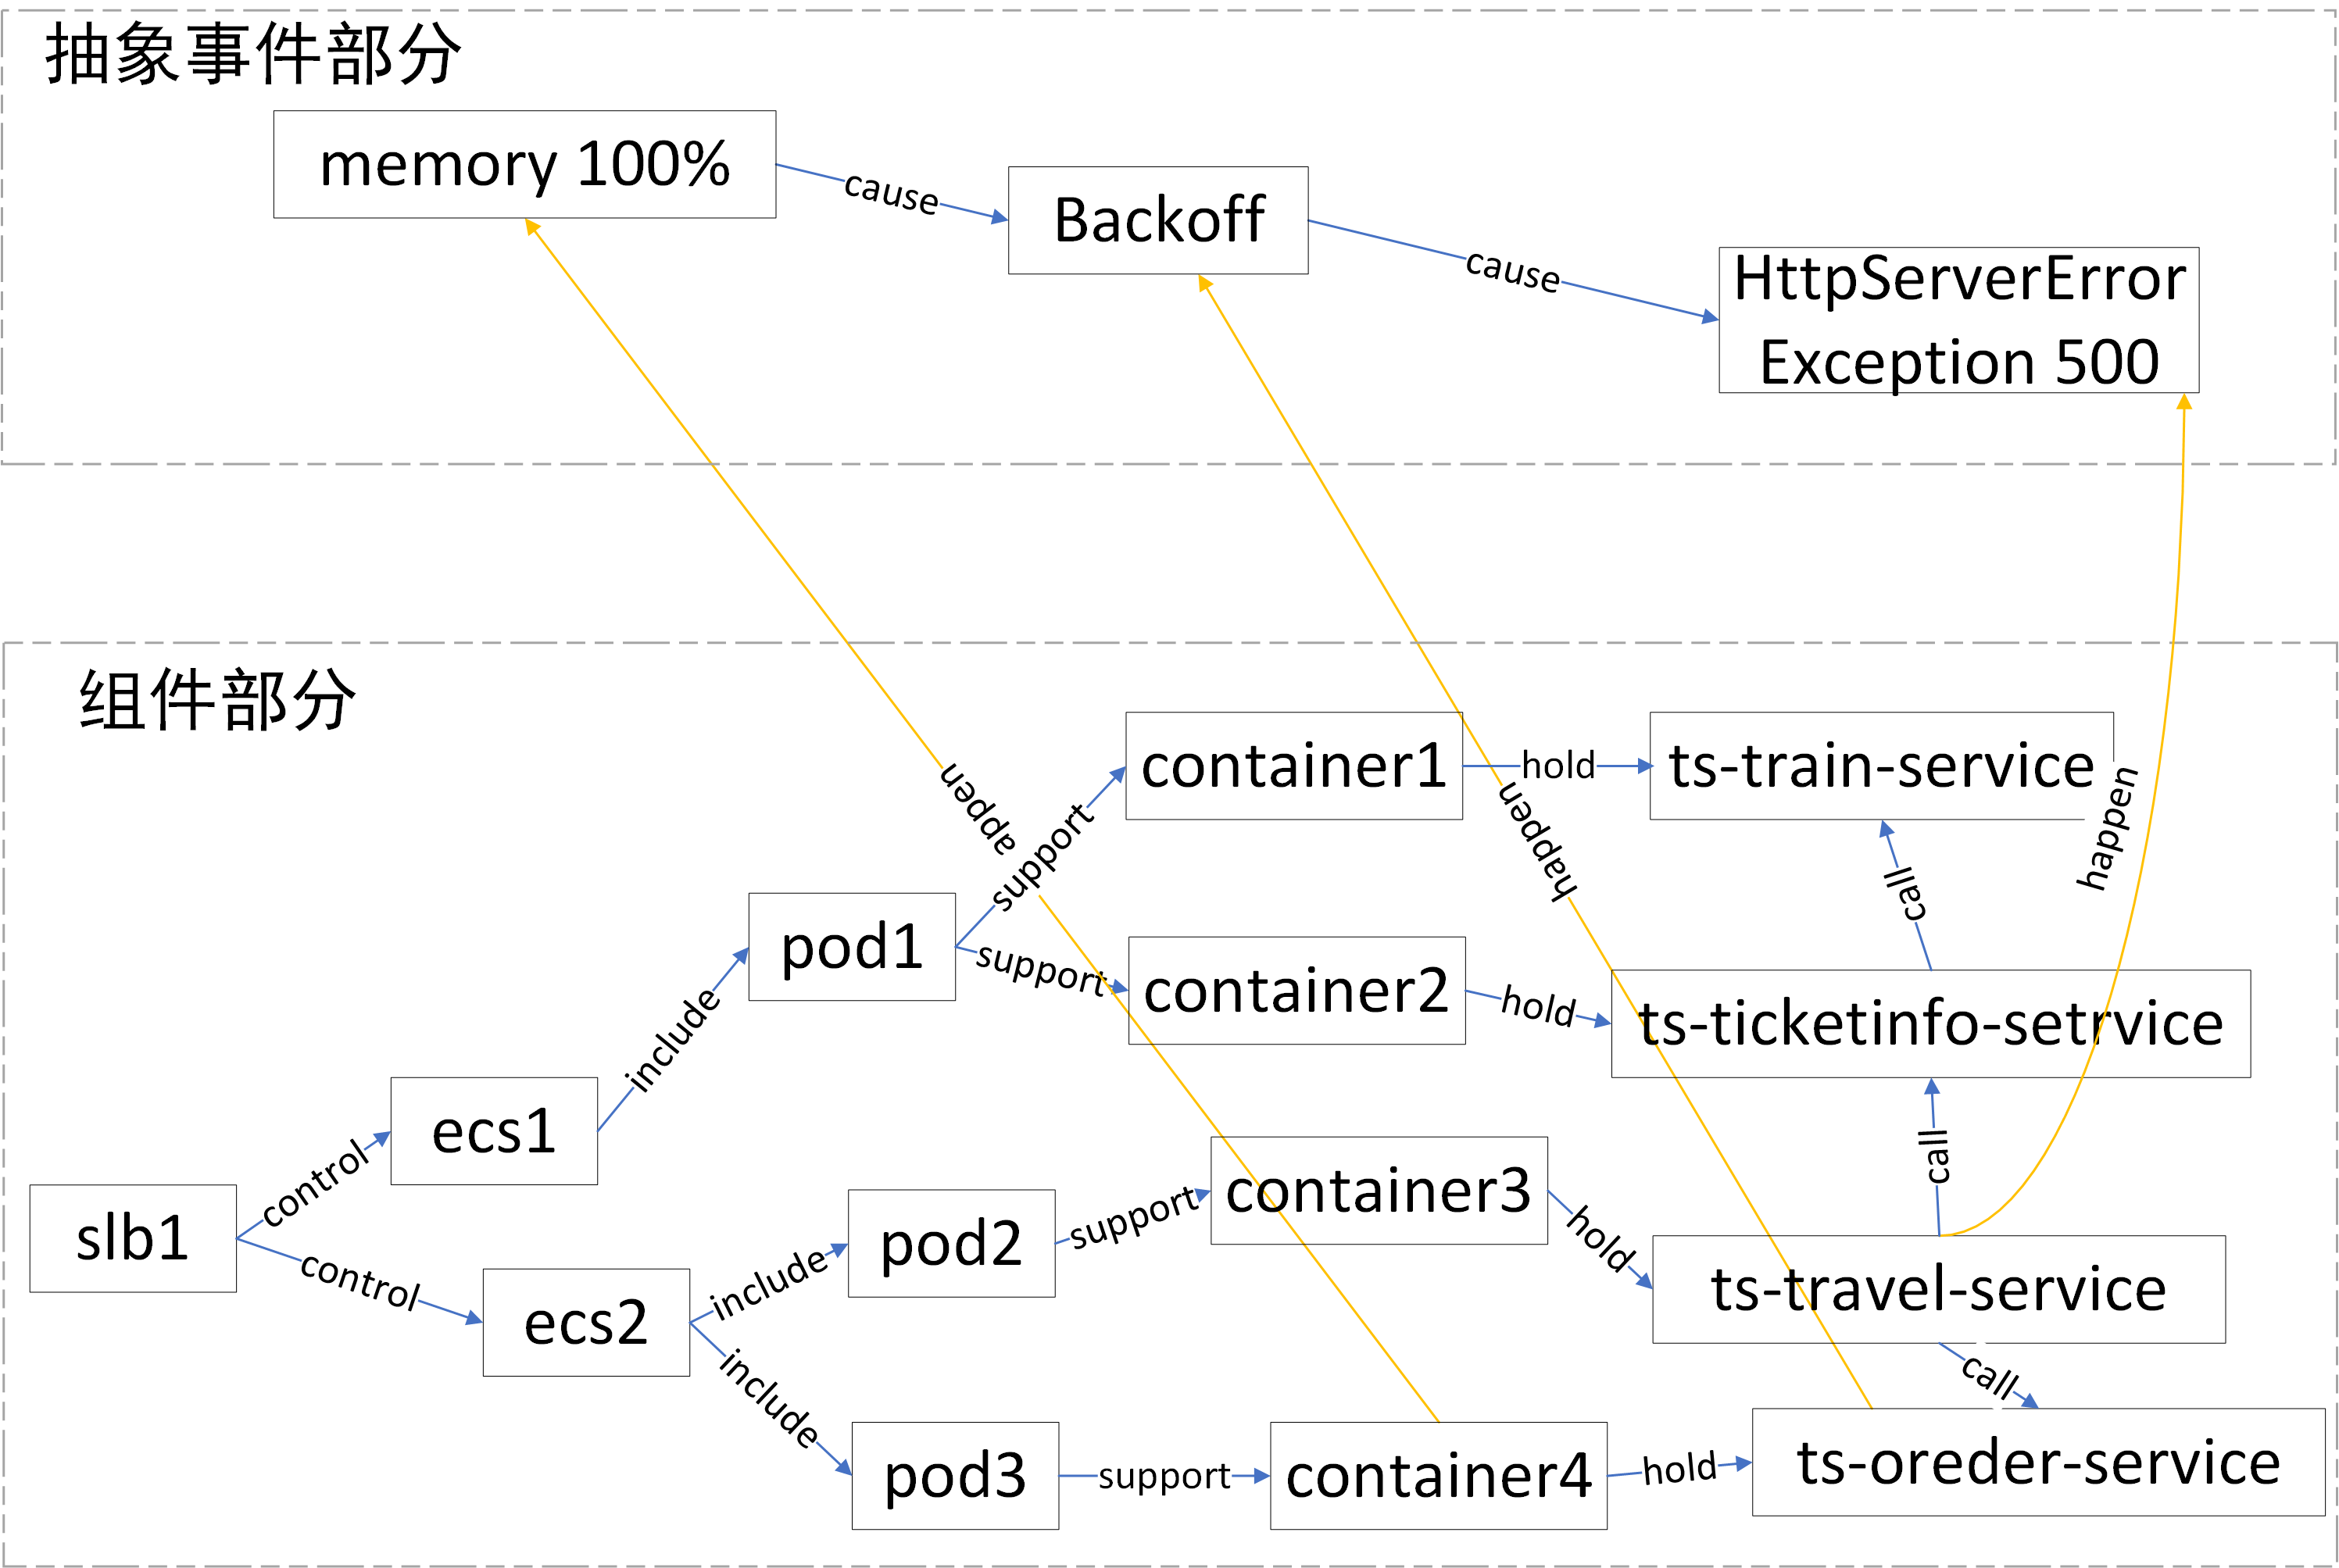
\includegraphics[width=.7\textwidth]{order-service-error.png}
    \caption{订票服务不可用故障对应知识图谱部分示例\label{order-service-error}}
\end{figure}

根据上下文进行动态表示在词嵌入领域已经有大量的相关工作。在最初的工作中,word2vec\cite{mikolov2013efficient}最大化单词在上下文出现的概率,将每个单词表示为低维稠密的静态向量,却忽视了单词在不同上下文含义不同。为了识别单词在不同上下文中具体的语义,ELMo\cite{peters2018deep}提出使用双层记忆网络,Bert\cite{devlin2018bert}使用基于自注意力机制的Transformer\cite{vaswani2017attention}编码层以获取单词随上下文变动的动态词向量。其中Bert所使用的Transformer结构其实是将一段文本看做单词为结点的全连接图。

受此启发,本文可以将知识图谱看作稀疏有向图,使用关系图卷积神经网络作为编码器,获取实体的上下文图结构信息。
% 1.rgcn后面连接的解码器什么样子
% 2.loss函数怎么计算 分类 关系 还是 头尾实体预测
% 3.模型的输入是什么

\section{组件-事件知识图谱动态表示学习模型}
上文介绍到实体会出现在不同的上下文中,所以需要随着上下文的变化拥有动态的向量表示。由于RGCN可以充分提取图的拓扑结构信息,所以本文使用RGCN作为编码器,获取实体的上下文图结构信息。在RGCN部分,为了让实体对不同的邻居结点有不同的侧重,本文又引入了注意力机制给邻居结点赋予了不同的权重,即Attention-RGCN。

本节详细介绍了针对组件-事件知识图谱的表示学习方法,分为模型结构、优化目标和预测3小节。
\subsection{模型结构}
整个模型结构如图\ref{kg-representation}所示,可见主要包括嵌入层、Attention-RGCN层、三元组分类层、实体分类层和关系分类层。下面将会分别对每一层展开介绍。
\begin{figure}[htbp]
    \centering
    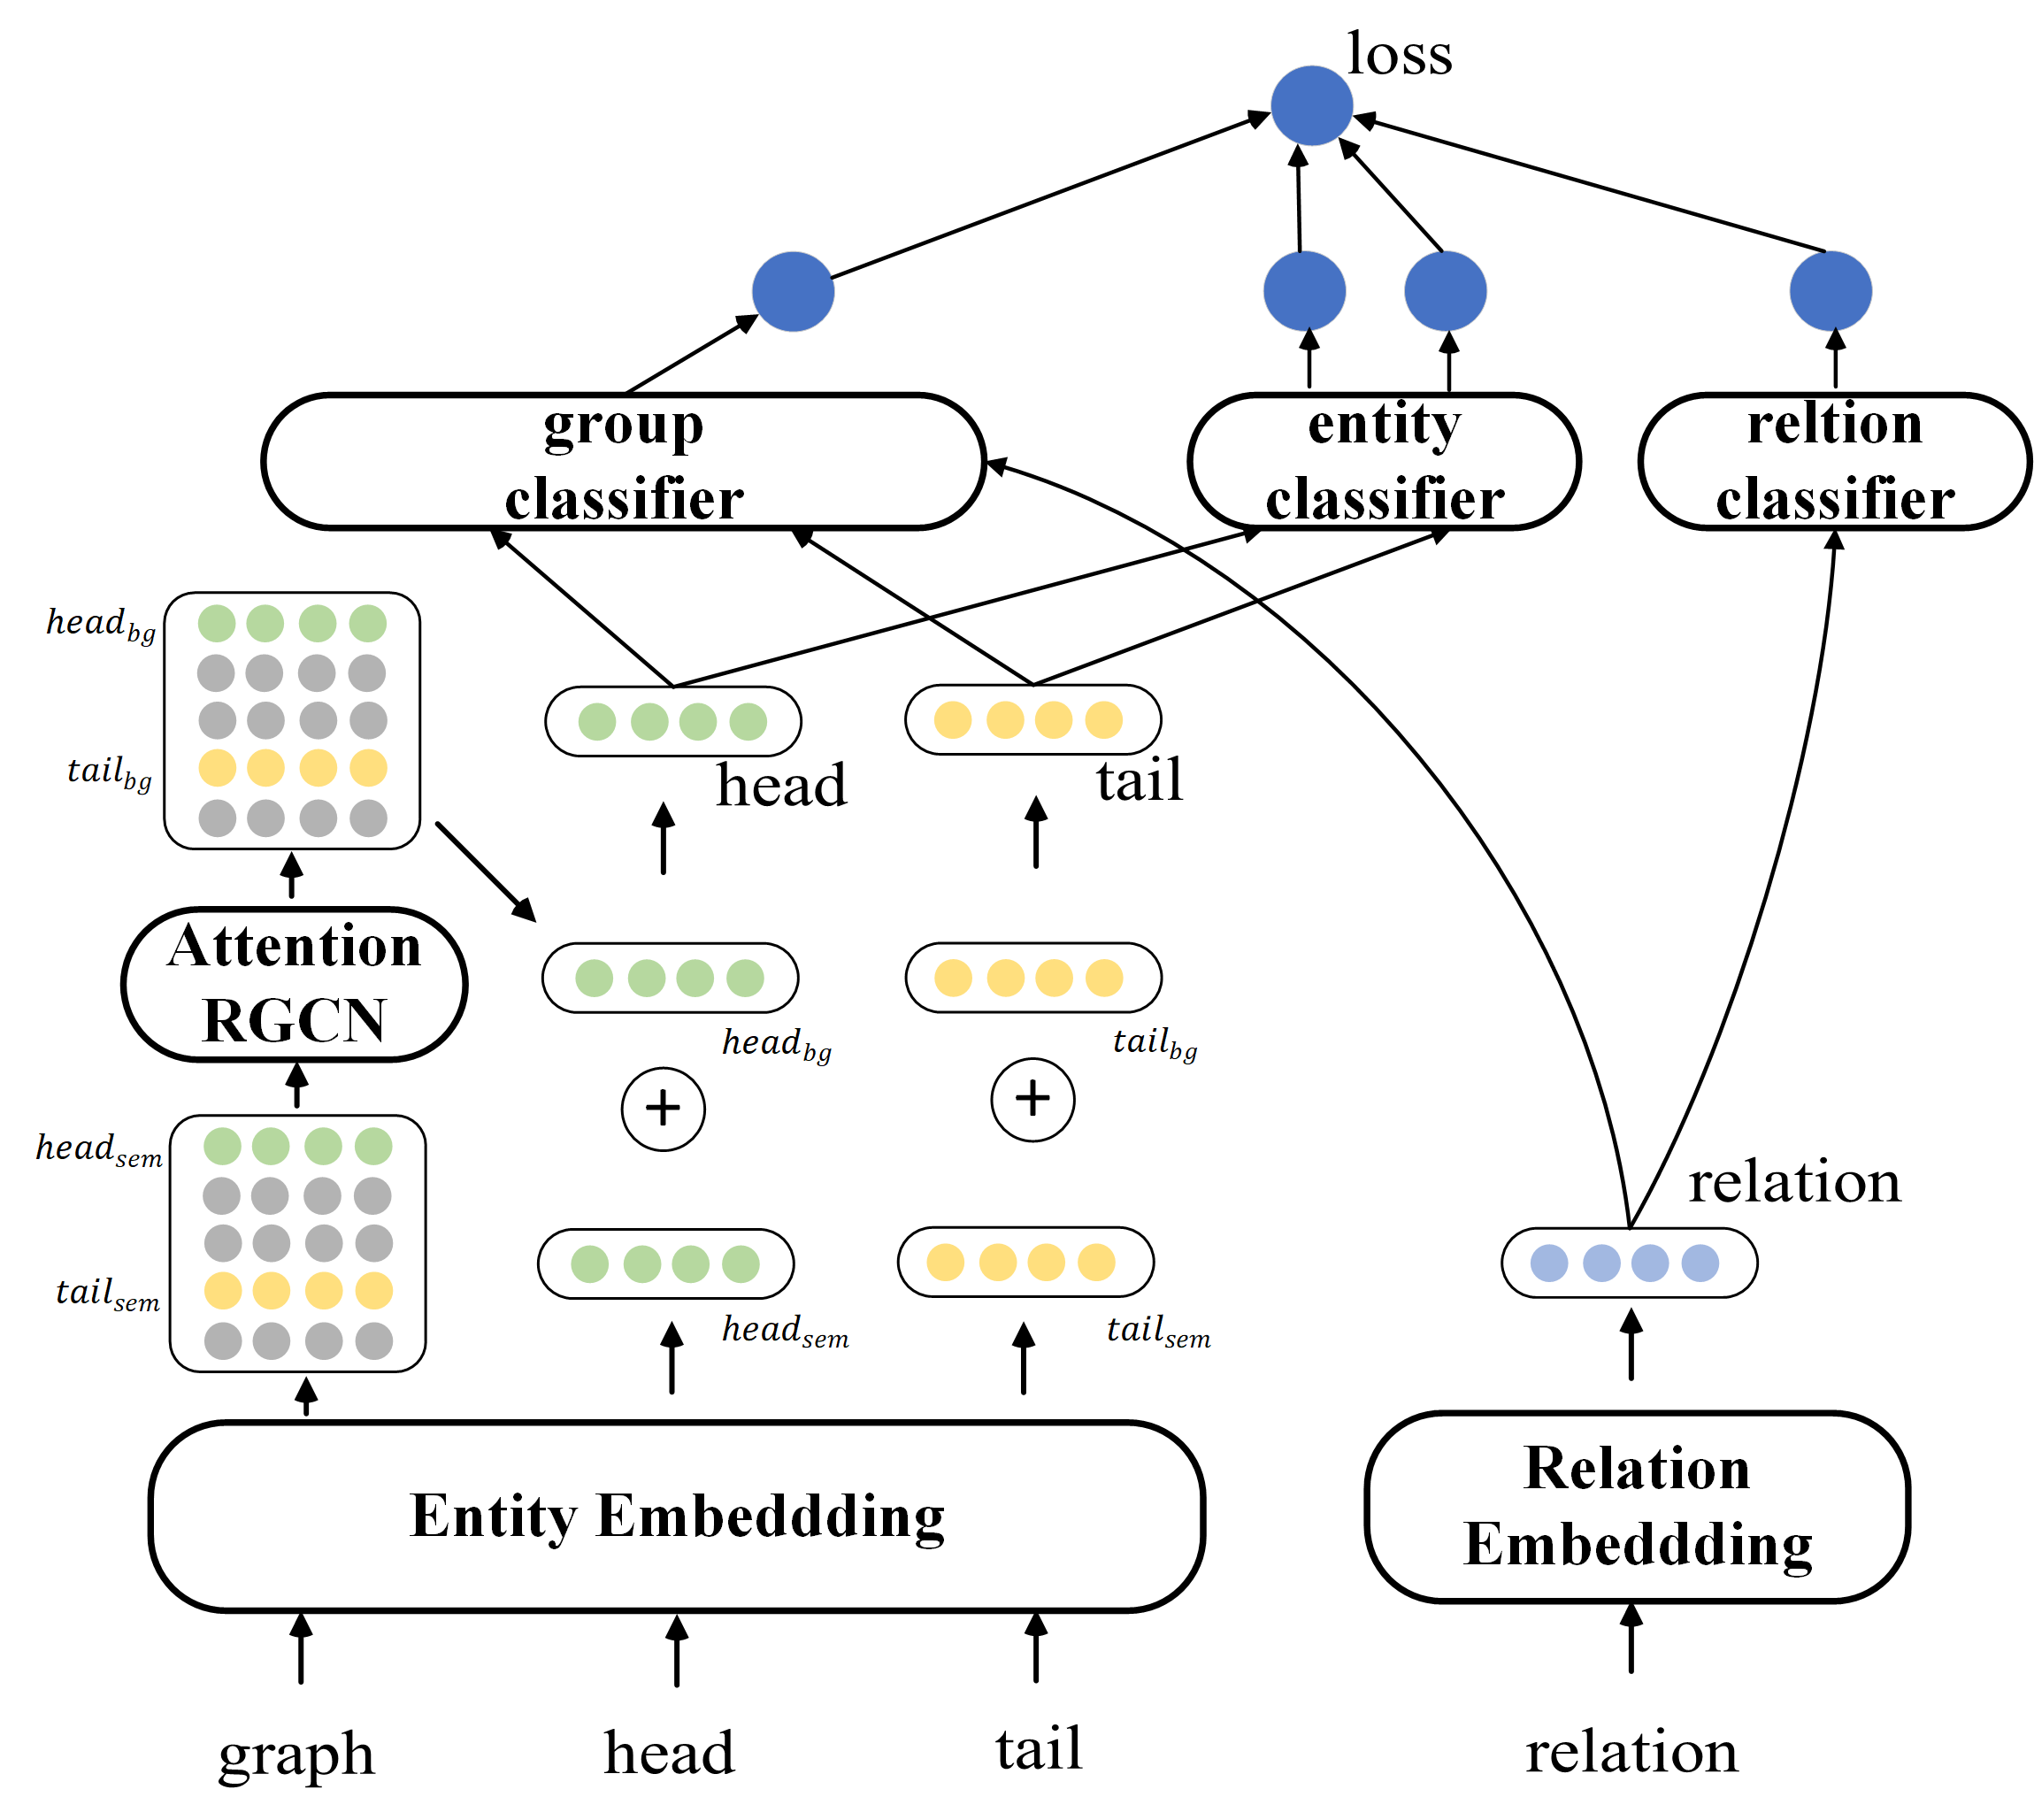
\includegraphics[width=.65\textwidth]{kg-representation.png}
    \caption{组件-事件知识图谱表示学习模型\label{kg-representation}}
\end{figure}

在嵌入层,模型的输入除了三元组$(head, relation, tail)$还有该三元组所在的上下文图$graph$,即$(graph, head,rlation,tail)$。在输入数据前,若三元组为$graph$中存在的,会将$graph$中$head$与$tail$之间的关系$relaion$去掉,防止引入的图结构信息$head_{bg}$与$tail_{bg}$包含了$relation$信息;若三元组中$head$或$tail$不存在于$graph$中,则对应$head_{bg}$或$tail_{bg}$设置为全零。在输入数据后,数据被嵌入层转化为初步向量表示,$graph$被转为了张量矩阵,$head$、$relation$、$tail$则都被转为了单维的向量。初始的嵌入层向量来自于实体、关系的语义信息。具体实现上,使用文本类的日志数据对Bert\cite{devlin2018bert}进行预训练,然后每个实体或关系的初始特征向量使用其分词后多个单词的向量均值。

Attention-RGCN层主要在RGCN模型中引入了注意力机制。章节\ref{RGCN}已经对RGCN进行了介绍,在进行特征传播时,实体对其上下文实体都赋予了相同的权重。但在组件-事件知识图谱中,实体对其上下文邻居实体是有不同侧重的,如图\ref{graph-example}中$cpu 100\%$和$memory 100\%$导致了$Backoff$的发生,但$memory 100\%$对$Backoff$的发生更具关键性,它意味着$container1$中没有足够的内存满足$ts-train-service$配置文件里规定的启动需求。因此,本文将注意力机制引入图卷积网络的传播过程,如式\ref{attention-rgcn}所示。
\begin{equation}
    h_{i}^{(l+1)}=\sigma\left(\sum_{r \in \mathcal{R}} \sum_{j \in \mathcal{N}_{i}^{r}} \alpha_{(j, r, i)} \frac{1}{c_{i, r}} W_{r}^{(l)} h_{j}^{(l)}+W_{0}^{(l)} h_{i}^{(l)}\right)
    \label{attention-rgcn}
\end{equation}
整体结构与式\ref{propo-in-directedgraph}一致,其中新引入的$\alpha_{(j, r, i)}$目的在于计算第$i$个结点对其在关系$r$下的邻居结点$j \in \mathcal{N}_{i}^{r}$的注意力权重。其计算公式如下:
\begin{equation}
    v_{(j, r, i)}=\mathbf{W_a}^{T}\left(\mathbf{W_e} h_{j}+\mathbf{W_r} h_{r} + \mathbf{W_e} h_{i}\right)
    \label{group-loss-part1}
\end{equation}
\begin{equation}
    \alpha_{(j, r, i)}=\operatorname{softmax}\left(v_{(j, r, i)}\right)=\frac{\exp \left(v_{(j, r, i)}\right)}{\sum_{j^{\prime} \in \mathcal{N}_{i}^{r}} \exp \left(v_{\left(j^{\prime}, r, i\right)}\right)}
    \label{group-loss-part2}
\end{equation}
式\ref{group-loss-part1}中$h_i,h_j,h_r\in\mathbb{R}^{d}$,$\mathbf{W_a}\in \mathbb{R}^{d}$,$\mathbf{W_e},\mathbf{W_r} \in \mathbb{R}^{d\times d}$是注意力参数矩阵。最终得到的$ v_{(j, r, i)} \in \mathbb{R}$即为索引为$i$的结点对关系$r$下索引为$j$的结点的注意力权重值。式\ref{group-loss-part2}使用$softmax(.)$函数进一步规范化注意力权重值,其中$\mathcal{N}_{i}^{r}$为索引为$i$的结点在关系$r$下对应的实体索引值集合。经过Attention-RGCN层后可以得到$head$、$tail$对应的上下文图结构嵌入表示$head_{bg}$、$tail_{bg}$,再与通过初步嵌入层的语义向量$head_{sem}$、$tail_{sem}$累加即可得到同时融入了语义信息和上下文图结构信息的嵌入表示$head_{new}$、$tail_{new}$。

实体分类器用于对实体进行分类,类别标签包括$contanier$、$event$、$service$等共计$c_{n}$个。输入为经过Attention-RGCN得到的融合了语义及上下文图结构信息的嵌入表示$head_{new}$、$tail_{new}$。随后将$head_{new}$、$tail_{new}$输入$d \times h \times c_{n}$的多层感知机和$softmax(.)$层,即可得到实体对各类分类情况。损失函数使用交叉熵,如式\ref{my_entity_loss}所示。其中,$i$、$j$对应着$head$、$tail$两实体的索引号,$h_i$、$h_j$为两实体在网络模型中的输出,$y_i$、$y_j$为两实体的标注向量,$k$表示向量第$k$维度。
\begin{equation}
    \mathcal{L}_{entity}= - \sum_{k=1}^{K} y_{i k} \ln h_{i k} - \sum_{k=1}^{K} y_{j k} \ln h_{j k}
    \label{my_entity_loss}
\end{equation}

关系分类器用于对关系向量分类,类别包括$cause$、$happen$、$hold$等。与实体分类一样,使用多层感知机、$softmax(.)$层分类,然后损失函数使用交叉熵即可,如式\ref{my_relation_loss}所示。其中,$h_r$为关系对应的网络输出向量,$y_r$为关系的标注向量,$k$表示向量第$k$维度。
\begin{equation}
    \mathcal{L}_{relation}=- \sum_{k=1}^{K} y_{r k} \ln h_{r k}
    \label{my_relation_loss}
\end{equation}

三元组分类器用于判别三元组是否存在,可以使用文献\parencite{trouillon2016complex}中形如式\ref{attention-rgcn-group-score}的评分函数。其中$\operatorname{diag}\left(.\right)$将$h_r\in\mathbb{R}^{d}$中每一个元素当作二维矩阵的对角线元素,从而得到$\mathbb{R}^{d}\times \mathbb{R}^{d}$的二维矩阵。损失函数使用交叉熵,如式\ref{my_group_loss}所示,其中$\mathcal{T}$表示所有的输入$(g, i, r, j)$集合,$l(.)$为激活函数,$y$为三元组是否成立的标签。
\begin{equation}
    f(h_{j}, h_{r}, h_{i})=h_{j}^{T} \operatorname{diag}\left(h_{r}\right) h_{i}
    \label{attention-rgcn-group-score}
\end{equation}

\begin{equation}
    \mathcal{L}_{group}= -\frac{1}{|\mathcal{T}|}  \sum_{(g, i, r, j) \in \mathcal{T}} y \log l(f(h_i, h_r, h_j))+(1-y) \log (1-l(f(h_i, h_r, h_j)))
    \label{my_group_loss}
\end{equation}

\subsection{优化目标}\label{representation-paras-learn}
根据上一小节所述,本模型的损失函数为实体分类器、关系分类器、三元组分类器三部分损失函数之和。最终本模型的损失函数如式\ref{represent-loss-all}所示:

\begin{equation}
    \begin{aligned}
    \mathcal{L}=-\frac{1}{|\mathcal{T}|}&  \sum_{(g, i, r, j) \in \mathcal{T}} y \log l(f(h_i, h_r, h_j))+(1-y) \log (1-l(f(h_i, h_r, h_j)))\\
    &- \sum_{k=1}^{K} y_{i k} \ln h_{i k} - \sum_{k=1}^{K} y_{j k} \ln h_{j k}\\
    &- \sum_{k=1}^{K} y_{r k} \ln h_{r k}\\
    \end{aligned}
    \label{represent-loss-all}
\end{equation}

\subsection{预测}
对组件-事件知识图谱进行表示学习后,可以进行抽象事件预测(预测在已发生抽象事件情况下是否会在某组件上发生某种事件)。本质上,就是在给定上下文图结构$g$下,三元组$(i, r, j)$是否成立。

将上下文图结构、头实体、关系和候选尾实体$g$、$(i, r, j)$输入表示学习模型中,会得到该三元组成立的评分,将评分最高的三元组对应的尾实体作为预测抽象事件即可,如式\ref{predict-next-event}所示。

\begin{equation}
    e = \mathop{\arg\max}\limits_{j\in events}( f (h_i, h_r, h_j)) 
    \label{predict-next-event}   
\end{equation}


\section{实验与分析}\label{representation-experiment}
在本节中,对本章提出的组件-事件知识图谱表示学习模型进行了实验与分析。
\subsection{数据集构建}
如实际运维场景一样,本文将模拟收集的数据划分成了历史数据和实时数据。具体上,模拟收集的所有数据会首先按照故障类型分组。然后,每种故障类型下的时间段集合会被划分成历史故障数据和实时故障数据,如表\ref{anomal-split}所示。

根据章节\ref{event-cause-classidier-experiment}事件因果关系判别实验结果,本处选用SVM模型从每类故障对应的历史故障数据中挖掘事件因果对,再按照章节\ref{graph-generate}所示步骤沉淀生成每类故障的组件-事件知识图谱。由模型初步生成的知识图谱虽然满足了实际使用需求,但不能保证没有任何瑕疵。因此,后续运维专家参与了知识图谱调优,保证了知识图谱绝对无瑕。在调优过程中,因为本文方法初步生成的知识图谱含有实体、关系量级低,所以知识图谱调优过程消耗人工较少。
\begin{table}[htbp]
    \caption{模拟数据划分}
    \centering
    \label{anomal-split}
    \begin{tabular}{cccc}
    \toprule[2pt]
                分布式应用 & \begin{tabular}[c]{@{}c@{}}模拟故障\\ 时间段总数\end{tabular} & \begin{tabular}[c]{@{}c@{}}历史故障\\ 时间段数\end{tabular} & \begin{tabular}[c]{@{}c@{}}实时故障\\ 时间段数\end{tabular} \\ \midrule[2pt]
    train-ticket & 471                                                  & 325                                                 & 146                                                 \\
    sock-shop    & 539                                                  & 371                                                 & 168                                                 \\ \bottomrule[2pt]
    \end{tabular}
\end{table}

\begin{table}[htbp]
    \caption{各类故障对应知识图谱信息}
    \centering
    \label{kg-abstract-event-num}
    \begin{tabular}{cccc}
    \toprule[2pt]
    分布式应用          & 故障代号                                    & 抽象事件节点数目 & 抽象事件因果关系数目 \\ \midrule[2pt]
                 & f1                                      & 41       & 285        \\
                 & f2                                      & 39       & 297        \\
                 & f3                                      & 6        & 8          \\
                 & f5                                      & 62       & 81         \\
    train-ticket & f6                                      & 34       & 233        \\
                 & f10                                     & 15       & 51         \\
                 & f13                                     & 15       & 15         \\
                 & f16                                     & 35       & 59         \\
                 & f17                                     & 38       & 65         \\
                 & f18                                     & 54       & 88         \\ \midrule[1pt]
                 & db\_goods\_disappeared                  & 20       & 86         \\
                 & db\_cart\_disappeared                   & 70       & 638        \\
                 & user\_unable\_log\_in                   & 52       & 180        \\
                 & db\_order\_disappeared                  & 20       & 114        \\
                 & order\_cart\_500                        & 9        & 8          \\
                 & order\_count\_500                       & 55       & 536        \\
                 & order\_payment\_500                     & 13       & 30         \\
                 & user\_register\_500                     & 7        & 6          \\
    sock-shop    & cart\_disappeared                       & 4        & 5          \\
                 & catalogue\_goods\_disappeared           & 6        & 7          \\
                 & add\_cart\_delay                        & 30       & 57         \\
                 & user\_register\_and\_log\_in\_delay     & 17       & 43         \\
                 & check\_order\_delay                     & 102      & 598        \\
                 & net\_loss\_check\_order                 & 92       & 614        \\
                 & net\_loss\_add\_cart                    & 34       & 79         \\
                 & net\_loss\_user\_register\_and\_log\_in & 17       & 55         \\
                 & net\_loss\_goods\_appear\_delay         & 15       & 33         \\ \bottomrule[2pt]
    \end{tabular}
\end{table}

\begin{table}[htbp]
    \centering
    \caption{知识库三元组数目及划分}
    \label{triple-split}
    \begin{tabular}{cccccccc}
    \toprule[2pt]
    分布式应用        & \begin{tabular}[c]{@{}c@{}}组件层\\ 三元组数\end{tabular} & \begin{tabular}[c]{@{}c@{}}组件-事件间\\ 三元组数\end{tabular} & \begin{tabular}[c]{@{}c@{}}事件层\\ 三元组数\end{tabular} & \begin{tabular}[c]{@{}c@{}}总\\ 三元组数\end{tabular} & 训练集  & 验证集 & 测试集 \\ \midrule[2pt]
    train-ticket & 1469                                               & 339                                                   & 1182                                               & 2990                                             & 1794 & 598 & 598 \\
    sock-shop    & 1043                                               & 563                                                   & 3089                                               & 4695                                             & 2817 & 939 & 939 \\ \bottomrule[2pt]
    \end{tabular}
    \end{table}
\newpage
表\ref{kg-abstract-event-num}统计了两个分布式应用每类故障类型所对应组件-事件知识图谱的抽象事件实体数目及抽象事件因果关系对数。在每张组件-事件知识图谱中,由于每个抽象事件实体都对应着一个组件实体,所以组件到抽象事件的发生关系数量与抽象事件节点数相等;由于组件层实体数量和关系数量只与分布式应用有关,所以每个组件-事件知识图谱的组件层关系数是恒定的。train-ticket组件层关系数为1469,sock-shop组件层关系数为1043。

在知识图谱中,一个关系对应着一个三元组,所以直接将各个组件-事件知识图谱中的每个关系对应的三元组视作正样本,即将其标注为“成立”。其中组件层的关系不会被重复使用,防止数据不均衡。表\ref{triple-split}为本块实验使用的正样本三元组数量,和按照6:2:2划分数据集的结果。另外,对于每一个正样本三元组,可以将其首实体或尾实体随机替换为不匹配的实体,构成负样本三元组,即“不成立”的三元组。
% 随后的实验中,数据的输入形式为三元组$(head,relation,tail)$及其所在上下文图结构$graph$。


\subsection{评测指标}
在知识图谱表示学习模型评测方式中有两个被广泛使用的任务。

\textbf{任务1}:链接预测,即预测受损三元组中缺少的头或尾实体。文献\parencite{bordes2011learning,bordes2013translatingE}定义链接预测为给定$(head,relation)$或$(relation,tail)$预测对应丢失的$tail$或$head$。在具体进行链接预测任务时,实验会排序候选实体集合,而不是直接只输出一个最佳匹配实体。

具体上,依据文献\parencite{bordes2013translatingE}的做法,对于每一个测试三元组$(head,relation,tail)$,实验会使用实体集合中任意不匹配$(relation,tail)$(或$(head,relation)$)的实体来替换$head$(或$tail$)生成受损三元组,然后根据模型输出的三元组成立概率分数降序排列这些三元组。在获得所有三元组排名后,实验使用了两个衡量指标:正确实体的平均排名(即MR,mean rank);正确实体在前N名的占比(即Hits at n,Hits@n)。MR越小,Hits@N越大,都意味着表示模型效果越好。另外,文献\parencite{bordes2013translatingE}发现生成的受损三元组可能是正确三元组,所以需要将该三元组筛选过滤掉。而本文中,由于知识图谱已被调优过,每个正确三元组都在对应$graph$中完备地存在着,当实体与$(relation,tail)$(或$(head,relation)$)不匹配时(不存在于组件-事件知识图谱中)意味着其生成的受损三元组一定是错误的,所以本块实验不需进行过滤操作。
% 最终,train-ticket中每个正确三元组会生成1404个受损三元组,sock-shop中每个正确三元组会生成1238个受损三元组。

\textbf{任务2}:三元组分类,即判断给定的三元组是否是知识图谱中真实存在的。在三元组分类任务中,给定知识图谱$graph$和三元组$(head,relation,tail)$,需要判断它是否是正确的。该任务已经在已有的工作\parencite{bordes2013translatingE,wang2014knowledge,lin2015learning}中展开过,也被广泛的应用在很多自然语言处理场景,比如问答。

链接预测时,输入候选实体和上下文信息,输出三元组成立的概率,成立概率值越大排名越高,再计算对应的MR和Hits@N即可。三元组分类时,输入待测三元组及其上下文,输出该三元组是否成立,再计算精确率(precision)、召回率(recall)和F1值即可。


% 我们首先对标准链路预测任务中的不同嵌入模型进行了比较研究,即预测不可见三胞胎的正确性。如(Bordes et al.,2013b)中所述,我们将链接预测作为实体排序任务。对于测试数据中的每个三元组,我们依次将每个实体作为要预测的目标实体。计算字典中正确实体和所有损坏实体的分数,并按降序排列。我们考虑平均倒数秩(MRR)(一个回答实体的倒数秩在所有测试三元组上的平均值),命中@10(前10名精度)和平均精度(MAP)(如(Chang等人,2014年)中所用)作为评估指标(from EMBEDDING ENTITIES AND RELATIONS FOR LEARN-
% ING AND INFERENCE IN KNOWLEDGE BASES
% )
\subsection{实验方法}
本块实验选取了多个对比方法以验证本文模型的优越性。实验记录了选取的每个方法在上小节两个评测任务上的表现指标。所选取的各个方法如下所示:
\begin{itemize}
    \item [(1)] 
    \textbf{TransE}\cite{bordes2013translatingE}:TransE将每个三元组(head,relation,tail)中的relation视作从head到tail的翻译过程。
    \item [(2)]
    \textbf{TransH}\cite{wang2014knowledge}:TransH将头尾实体都投影到关系所在的张量空间中,可以解决复杂的一对多、多对多关系。
    \item [(3)]
    \textbf{TransR}\cite{lin2015learning}:TransR将关系也嵌入为矩阵,可以区分具有不同语义的关系。
    \item [(4)]
    \textbf{GAKE}\cite{feng2016gake}:GAKE引入邻居上下文、边上下文、路径上下文信息,可以捕获图结构的语义。
    \item [(5)]
    \textbf{TCE}\cite{shi2017knowledge}:TCE引入了两种结构信息,一种是实体的相邻实体,另一种是一对实体之间的关系路径。
    \item [(6)]
    \textbf{本文表示学习方法}:本文在章节\ref{chapter-3}所提出的组件-事件知识图谱表示学习模型。
    \item [(7)]
    \textbf{本文表示学习方法-1}:相比本文表示学习方法,去除了Attention-RGCN层的注意力机制。
    \item [(8)]
    \textbf{本文表示学习方法-2}:相比本文表示学习方法,去除实体分类模块的损失。
    \item [(9)]
    \textbf{本文表示学习方法-3}:相比本文表示学习方法,去除关系分类模块的损失。
  \end{itemize}

其中,TransE、TransH和TransR将每个三元组视作一条独立的知识,用于对比验证引入上下文结构信息对表示学习的提升;GAKE、TCE引入上下文结构信息获取静态表示向量,用于对比验证动态表示学习的有效性;\textbf{本文表示学习方法-1}使用无attention机制的RGCN,用于对比验证本文在RGCN中引入注意力机制的提升;\textbf{本文表示学习方法-2}去除实体分类模块,用于对比验证引入实体类别信息对模型的提升;\textbf{本文表示学习方法-3}去除关系分类模块,用于对比验证关系类别信息对模型的提升。

\subsection{实验结果与分析}
% \begin{table}[htbp]
%     \centering
%     \caption{链接预测结果}
%     \label{link-predict-result}
%     \begin{tabular}{ccccc}
%     \hline
%     方法     & MRR         &             & HIT@10        & H10 raw       \\ \hline
%     TransE & 125         & 243         & 47.1          & 34.9          \\
%     TransH & 84          & 211         & 58.5          & 42.5          \\
%     TransR & 77          & 198         & 68.7          & 48.2          \\
%     GAKE   & 119         & 228         & 64.8          & 44.5          \\
%     TCE    & 25          & 110         & 83.1          & 55.3          \\
%     本文方法   & \textbf{17} & \textbf{86} & \textbf{85.4} & \textbf{59.4} \\
%     本文方法-1 & 24          & 124         & 82.6          & 52.1          \\ \hline
%     \end{tabular}
% \end{table}
% \begin{table}[htbp]
%     \caption{链接预测结果}
%     \centering
%     \label{link-predict-result}
%     \begin{tabular}{ccc}
%     \hline
%     方法     & MR                          & Hits@3                         \\ \hline
%     TransE & 121                          & 48.3                           \\
%     TransH & 83                           & 57.3                           \\
%     TransR & 71                           & 66.2                           \\
%     GAKE   & 76                           & 62.8                           \\
%     TCE    & 32                           & 81.9                           \\
%     本文方法   & \textbf{17} & \textbf{85.4} \\
%     本文方法-1 & 24                           & 82.6                           \\ \hline
%     \end{tabular}
% \end{table}
\begin{table}[htbp]
    \caption{链接预测结果}
    \centering
    \label{link-predict-result}
    \begin{tabular}{ccccc}
    \toprule[2pt]
           & \multicolumn{2}{c}{train-ticket} & \multicolumn{2}{c}{sock-shop} \\
    方法     & MR            & Hits@5           & MR           & Hits@5         \\ \midrule[2pt]
    TransE & 59            & 48.3             & 63           & 42.7           \\
    TransH & 42            & 57.3             & 56           & 45.2           \\
    TransR & 37            & 66.2             & 43           & 59.8           \\
    GAKE   & 33            & 62.8             & 39           & 53.2           \\
    TCE    & 23            & 81.9             & 31           & 78.1           \\
    本文表示学习方法   & \textbf{9}    & \textbf{85.4}    & \textbf{13}  & \textbf{82.9}  \\
    本文表示学习方法-1 & 26            & 79.5             & 34           & 67.6         \\ 
    本文表示学习方法-2 & 19           & 82.2             & 30           & 78.4           \\ 
    本文表示学习方法-3 & 16            & 83.6            & 24           & 81.2          \\ 
    \bottomrule[2pt]
    \end{tabular}
\end{table}

\begin{table}[htbp]
    \caption{三元组分类结果}
    \centering
    \label{triple-class-result}
    \begin{tabular}{ccccccc}
    \toprule[2pt]
               &                & train-ticket   &                &                & sock-shop      &                \\
    方法         & precision      & recall         & F1             & precision      & recall         & F1             \\ \midrule[2pt]
    TransE     & 0.650          & 0.692          & 0.670          & 0.653          & 0.626          & 0.639          \\
    TransH     & 0.703          & 0.730          & 0.716          & 0.707          & 0.675          & 0.691          \\
    TransR     & 0.743          & 0.716          & 0.730          & 0.680          & 0.701          & 0.690          \\
    GAKE       & 0.781          & 0.749          & 0.765          & 0.722          & 0.742          & 0.732          \\
    TCE        & 0.804          & 0.783          & 0.793          & 0.736          & 0.769          & 0.752          \\
    本文表示学习方法   & \textbf{0.864} & \textbf{0.837} & \textbf{0.850} & \textbf{0.836} & \textbf{0.814} & \textbf{0.825} \\
    本文表示学习方法-1 & 0.763          & 0.816          & 0.788          & 0.776          & 0.746          & 0.761          \\
    本文表示学习方法-2 & 0.826          & 0.801          & 0.813          & 0.783          & 0.808          & 0.795          \\
    本文表示学习方法-3  & 0.845          & 0.822          & 0.834          & 0.788          & 0.810           & 0.799          \\ \bottomrule[2pt]
    \end{tabular}
\end{table}
在链接预测任务上,表\ref{link-predict-result}列出了各个方法的链路预测结果。\textbf{本文表示学习方法}在MR和Hit@5指标上都得到了比其他方法更好的实验结果。在三元组分类任务上,表\ref{triple-class-result}列出来各个方法的精确率(precision)、召回率(recall)和F1值。\textbf{本文表示学习方法}相较基线方法获得了5\%以上的F1值提升。实验结果证明了本文利用注意力机制的RGCN获取图结构上下文信息,再结合语义信息的动态表示学习方法,可以更好地嵌入表示组件-事件知识图谱。

对比\textbf{本文表示学习方法-1}、\textbf{本文表示学习方法-2}、\textbf{本文表示学习方法-3},可发现图神经网络的注意力机制对模型的提升效果最大,其可以强化重要信息的传播、挖掘重要的图结构信息;实体、关系类别信息的引入也可以改善知识表示学习效果,其中实体类别信息比关系类别信息重要性更高。

另外,\textbf{本文表示学习方法}在三元组分类任务上取得的精确率要比链接预测上Hits@5要高,原因在于三元组分类任务中每个“成立”的三元组都只生成$\omega$个“不成立”的受损三元组(本实验中$\omega$取100);而链接预测任务中,每个正确三元组与平均约1000个受损三元组进行比较排序。

本块实验中,本文模型达到最佳效果时使用的超参为:嵌入层维度为100;Attention-RGCN为4层、输入窗口大小为128节点,中间隐状态维度为50、输出隐状态维度为100;实体分类器结构为$100*32*7$,7为实体种类数;关系分类器结构为$100*32*8$,8为关系种类数。
\section{本章小结}
本章主要介绍了组件-事件知识图谱的表示学习模型,通过将实体表示分为结构特征和语义特征,其中拓扑结构特征通过Attention-RGCN获取,语义特征使用实体分词对应词向量均值表示,从而实现了实体在不同拓扑上下文的动态表示。同时也介绍了优化目标和预测事件的公式。实验结果验证了本章表示学习模型的有效性。

% 1、基于 h r t 三元组
% 相关工作:基于path的那种
% 本文:将上下文考虑进去,上下文要么 (hrt)集合  要么图(ve)
% loss:分类,三元组判别对不对
% 评判标准:链路预测、实体分类

% 2、基于 网络表示学习 的那种
% 相关工作:基于rgcn的那种
% 本文:将上下文考虑进去,上下文要么 (hrt)集合  要么图(ve)
% loss:分类,三元组判别对不对
% 评判标准:关系预测、结点分类



